\documentclass[a4paper,12pt]{article}
\usepackage[utf8]{inputenc}
\usepackage{graphicx}
\usepackage{fancyhdr}
\usepackage{amsmath}
\usepackage{adjustbox}
\usepackage{mathtools}
\usepackage{float}
\usepackage[spanish, es-nodecimaldot]{babel} 
\usepackage{lastpage}
\usepackage{amssymb} % Para símbolos matemáticos adicionales
\usepackage{hyperref}
\usepackage{cleveref}
%\usepackage[none]{hyphenat}
\usepackage{array}
\usepackage{listings}
\usepackage{xcolor}

\usepackage{multirow}
\usepackage{textcomp}
\usepackage[left=2.5cm, right=2.5cm, top=3cm, bottom=3cm]{geometry}

\lstset{ 
    language=Matlab,                     % El lenguaje del código
    basicstyle=\ttfamily,                % Tipo de letra
    keywordstyle=\color{blue},           % Color para palabras clave
    commentstyle=\color{green!60!black}, % Color para comentarios
    numbers=left,                        % Numeración de las líneas
    numberstyle=\tiny\color{gray},       % Estilo para los números
    stepnumber=1,                        % Mostrar número en cada línea
    tabsize=4,                           % Tamaño de tabulación
    breaklines=true,                     % Partir líneas largas
    showspaces=false,                    % No mostrar los espacios en blanco
    showstringspaces=false,              % No mostrar espacios dentro de strings
    showtabs=false,                      % No mostrar tabs
}

\graphicspath{{Imagenes/}}

% Encabezado y pie de página
\pagestyle{fancy}
\fancyhf{}
\setlength{\headheight}{30 pt}
\renewcommand{\headrulewidth}{0.2pt}
\fancyhead[R]{\begin{tabular}{@{}l@{}}
\includegraphics[scale=0.4]{escudo.PNG}\end{tabular}}
\fancyhead[L]{\begin{tabular}{@{}c@{}} \textbf{Robótica I - Año: 2024} \\ Trabajo Práctico 6: Jacobiano \end{tabular}}


\fancyfoot[R]{\thepage}
\fancyfoot[C]{\begin{tabular}{@{}c@{}}\textbf{BORQUEZ PEREZ Juan Manuel}\\ \textbf{Legajo 13567}\end{tabular}}
\renewcommand{\footrulewidth}{0.2pt}

\begin{document}

\begin{titlepage}
    \centering
    \vspace*{5cm}
    {\Huge\bfseries Informe de Trabajo Práctico N°6}\\
    \vspace{0.2cm}
    {\Large \textbf{Jacobiano}}\\
    \vspace{0.5cm}
    {\Large Robótica I}\\
    \vspace{0.5 cm}
    {\Large Ingeniería en Mecatrónica}\\
    \vspace{0.2 cm}
    {\Large Facultad de Ingeniería - UNCUYO}\\
    \vspace{1.5cm}
    Alumno: Juan Manuel BORQUEZ PEREZ\\
    Legajo: 13567\\
    \vfill
    {\begin{tabular}{@{}c@{}}
\includegraphics[scale=0.4]{escudo.PNG}\end{tabular}}\hspace{10pt}
    %Año 2023
\end{titlepage}

\section{Ejercicio 1}
\begin{figure}[H]
    \centering
    \begin{adjustbox}{scale = 0.55, max width=\columnwidth}
        \framebox{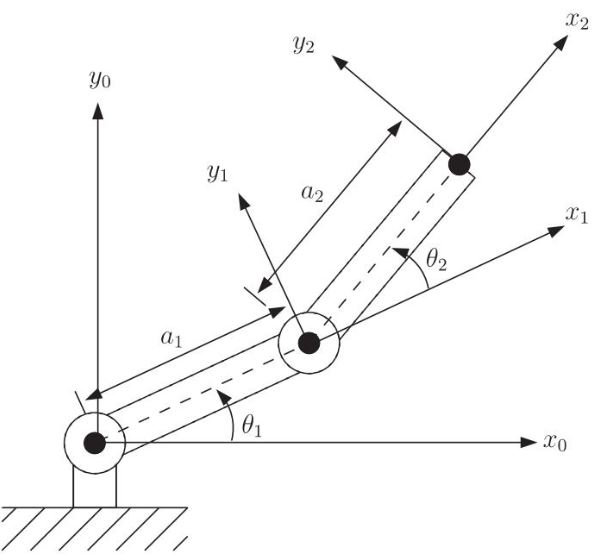
\includegraphics{1-Ejercicio_1.JPG}}
    \end{adjustbox}
    \caption{Robot planar RR Ejercicio 1.}
\end{figure}

\subsection{Mediante derivación respecto del tiempo obtenga el Jacobiano del robot}
Se tiene:

\begin{equation}
    \left\{
    \begin{aligned}
    x &= a_1 \cos(\theta_1) + a_2 \cos(\theta_1 + \theta_2) \\
    y &= a_1 \sin(\theta_1) + a_2 \sin(\theta_1 + \theta_2) \\
    z &= 0 \\
    \alpha &= 0 \\
    \beta &= 0 \\
    \gamma &= \theta_1 + \theta_2
    \end{aligned}
    \right.
    \label{directa RR}
\end{equation}

Cada fila en el Jacobiano se puede obtener como el gradiente de la función en esa fila
respecto de las variables $q_1\equiv\theta_1$ y $q_2\equiv\theta_2$. Se obtiene:

\begin{equation}
    J(q) = 
    \begin{bmatrix}
        -a_1\sin(\theta_1) - a_2\sin(\theta_1 + \theta_2) & -a_2\sin(\theta_1 + \theta_2)\\
        a_1\cos(\theta_1) + a_2\cos(\theta_1 + \theta_2)  & a_2\cos(\theta_1 + \theta_2)\\
        0                                                 & 0\\
        0                                                 & 0\\
        0                                                 & 0\\
        1                                                 & 1
    \end{bmatrix}
    \label{jacobiano RR}
\end{equation}

\subsection{Calcule la velocidad del extremo $\dot{p}$ , en m/s para $q = [\pi/6, \pi/6]$, en rad y $\dot{q}=
[0, -1]$ en rad/s. Suponga longitud de eslabón unitaria. Observe el gráfico del robot
e interprete los resultados}

Las velocidades en el extremo se calculan a partir de las velocidades articulares como:
\begin{equation}
    \dot{p} = J(q)\dot{q}
\end{equation}

Para los valores dados se obtiene:
\begin{equation*}
    \dot{p} = 
    \begin{bmatrix}
        -\sin(\pi/6) - \sin(\pi/3) & -\sin(\pi/3)\\
        \cos(\pi/6) + \cos(\pi/3)  & \cos(\pi/3)\\
        0                          & 0\\
        0                          & 0\\
        0                          & 0\\
        1                          & 1
    \end{bmatrix}
    \begin{bmatrix}
        0\\
        -1
    \end{bmatrix}
    =
    \begin{bmatrix}
        \sqrt{3}/2\\
        -1/2\\
        0\\
        0\\
        0\\
        -1
    \end{bmatrix}
    =
    \begin{bmatrix}
        0.866\\
        -0.500\\
        0.000\\
        0.000\\
        0.000\\
        -1.000
    \end{bmatrix}
\end{equation*}

En donde las primeras 3 componentes están en $m/s$ y las últimas 3 en $rad/s$.

\subsection{Trabaje solo con las coordenadas X-Y (primeras 2 filas del J) y verifique mediante la
inversa algebraica que $\dot{q} = J^{-1}(q)\dot{p}$ se cumple}

Conservando solo las filas del plano X-Y nos queda:

\begin{equation}
    J(q) = 
    \begin{bmatrix}
        -a_1\sin(\theta_1) - a_2\sin(\theta_1 + \theta_2) & -a_2\sin(\theta_1 + \theta_2)\\
        a_1\cos(\theta_1) + a_2\cos(\theta_1 + \theta_2)  & a_2\cos(\theta_1 + \theta_2)
    \end{bmatrix}
\end{equation}

Luego $J^{-1}(q)$ es:
\begin{equation}
    J^{-1}(q) =
    \begin{bmatrix}
        \frac{\cos(\theta_1 + \theta_2)}{a_1 \sin(\theta_2)} & \frac{\sin(\theta_1 + \theta_2)}{a_1 \sin(\theta_2)} \\
        -\frac{a_1 \cos(\theta_1) + a_2 \cos(\theta_1 + \theta_2)}{a_1 a_2 \sin(\theta_2)} & -\frac{a_1 \sin(\theta_1) + a_2 \sin(\theta_1 + \theta_2)}{a_1 a_2 \sin(\theta_2)}
    \end{bmatrix}
\end{equation}

Para los valores del inciso anterior verificamos:
\begin{equation*}
    J^{-1}(q)\dot{p} =
    \begin{bmatrix}
        \frac{\cos(\pi/3)}{\sin(\pi/6)} & \frac{\sin(\pi/3)}{\sin(\pi/6)} \\
        -\frac{\cos(\pi/6) + \cos(\pi/3)}{\sin(\pi/6)} & -\frac{\sin(\pi/6) + \sin(\pi/3)}{\sin(\pi/6)}
    \end{bmatrix}
    \begin{bmatrix}
        \sqrt{3}/2\\
        -1/2
    \end{bmatrix}
    = 
    \begin{bmatrix}
        0\\
        -1
    \end{bmatrix}
    = \dot{q}
\end{equation*}

\section{Ejercicio 3}
\textbf{halle el Jacobiano en forma general de los 3 robots siguientes}
\subsection{}

\begin{figure}[H]
    \centering
    \begin{adjustbox}{scale = 0.55, max width=\columnwidth}
        \framebox{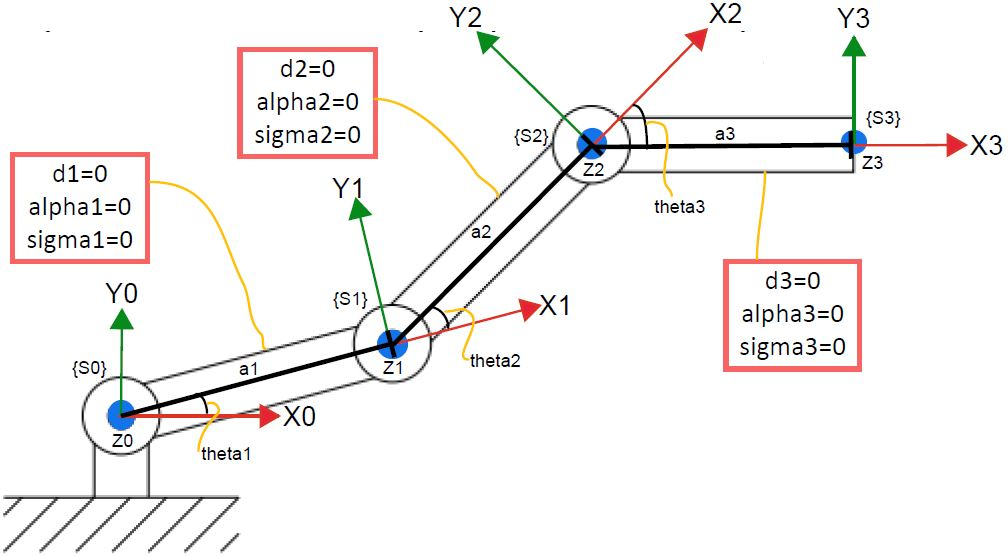
\includegraphics{2-Ejercicio_2_1_RR_DH.JPG}}
    \end{adjustbox}
    \caption{Convención DH utilizada para robot RRR planar.}
\end{figure}

Las ecuaciones de la cinemática directa se obtienen extendiendo las indicadas en \cref{directa RR} y se obtiene
\begin{equation*}
    \left\{
    \begin{aligned}
    x &= a_1 \cos(\theta_1) + a_2 \cos(\theta_1 + \theta_2) + a_3 \cos(\theta_1 + \theta_2 + \theta_3)\\
    y &= a_1 \sin(\theta_1) + a_2 \sin(\theta_1 + \theta_2) + a_3 \sin(\theta_1 + \theta_2 + \theta_3)\\
    z &= 0 \\
    \alpha &= 0 \\
    \beta &= 0 \\
    \gamma &= \theta_1 + \theta_2 + \theta_3
    \end{aligned}
    \right.
    \label{directa RRR}
\end{equation*}

El jacobiano se obtiene también por extensión de \cref{jacobiano RR}
\begin{equation}
    J(q) = 
    \begin{bmatrix}
        -a_1S_1 - a_2S_{12} - a_3S_{123}& -a_2S_{12} - a_3S_{123} & - a_3S_{123}\\
        a_1C_1 + a_2C_{12} + a_3C_{123}& a_2C_{12} + a_3C_{123}  &  a_3C_{123}\\
        0                               & 0                       & 0\\
        0                               & 0                       & 0\\
        0                               & 0                       & 0\\
        1                               & 1                       & 1
    \end{bmatrix}
    \label{jacobiano RRR}
\end{equation}

\subsection{}
\begin{figure}[H]
    \centering
    \begin{adjustbox}{scale = 0.55, max width=\columnwidth}
        \framebox{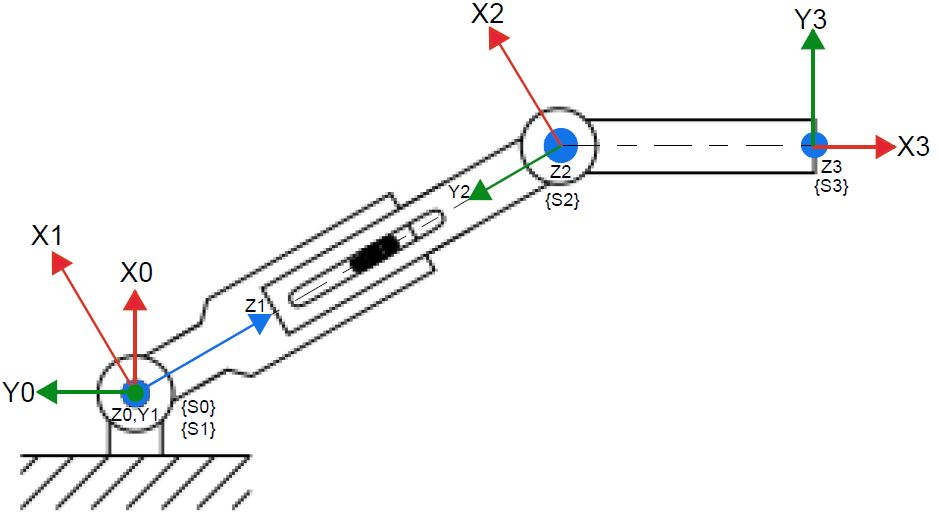
\includegraphics{3-Ejercicio_2_1_RLR_DH.JPG}}
    \end{adjustbox}
    \caption{Convención DH utilizada para robot RLR planar.}
\end{figure}

Los parámetros de DH del robot son:
\begin{table}[H]
    \centering
    \begin{tabular}{|c|c|c|c|c|c|}
    \hline
    Sistema & $\theta$          & $d$         & $a$         & $\alpha$     & $\sigma$ \\ \hline
    1       & $q_1$             & 0           & $0$         & $\pi/2$   & 0        \\ \hline
    2       & $0$               & $q_2$       & $0$         & $-\pi/2$  & 1        \\ \hline
    3       & $q_3$             & 0           & $a_3$  & $0$          & 0        \\ \hline
    \end{tabular}
    \caption{Parámetros DH RLR planar.}
\end{table}

Las ecuaciones de la cinemática directa se obtienen aplicando ``fkine'' de forma simbólica
en MATLAB:

\begin{equation*}
    CD = 
    \left[\begin{array}{cccc}
        \cos\left(q_{1}+q_{3}\right) & -\sin\left(q_{1}+q_{3}\right) & 0 & a_{3}\,\cos\left(q_{1}+q_{3}\right)+q_{2}\,\sin\left(q_{1}\right)\\
        \sin\left(q_{1}+q_{3}\right) & \cos\left(q_{1}+q_{3}\right) & 0 & a_{3}\,\sin\left(q_{1}+q_{3}\right)-q_{2}\,\cos\left(q_{1}\right)\\
        0 & 0 & 1 & 0\\
        0 & 0 & 0 & 1
    \end{array}
    \right]
\end{equation*}

Luego tenemos:
\begin{equation*}
    \left\{
    \begin{aligned}
    x &= a_{3}\,\cos\left(q_{1}+q_{3}\right)+q_{2}\,\sin\left(q_{1}\right)\\
    y &= a_{3}\,\sin\left(q_{1}+q_{3}\right)-q_{2}\,\cos\left(q_{1}\right)\\
    z &= 0 \\
    \alpha &= 0 \\
    \beta &= 0 \\
    \gamma &= q_1 + q_3
    \end{aligned}
    \right.
\end{equation*}

Finalmente el jacobiano es:

\begin{equation}
    J(q) = 
    \begin{bmatrix}
        -a_3\sin(q_1 + q_3) + q_2\cos(q_1) & \sin(q_1)  & -a_3\sin(q_1 + q_3)\\
        a_3\cos(q_1 + q_3)  + q_2\sin(q_1) & -\cos(q_1) & a_3\cos(q_1 + q_3)\\
        0 & 0 & 0\\
        0 & 0 & 0\\
        0 & 0 & 0\\
        1 & 0 & 1
    \end{bmatrix}
\end{equation}

\subsection{}

\begin{figure}[H]
    \centering
    \begin{adjustbox}{scale = 0.55, max width=\columnwidth}
        \framebox{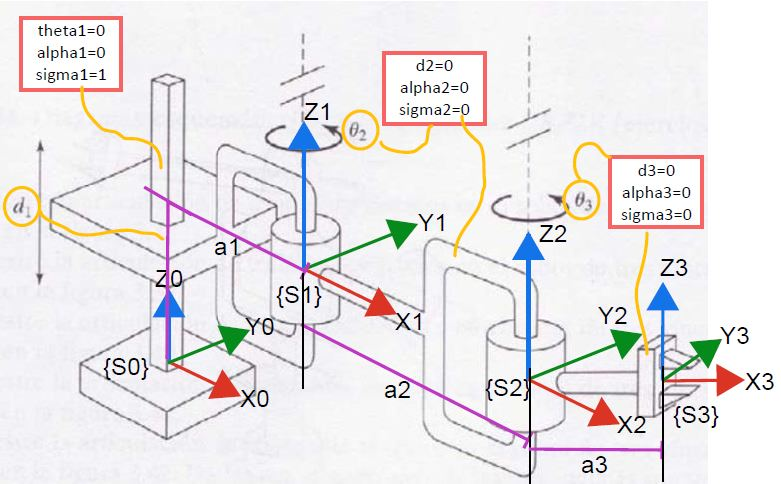
\includegraphics{4-Ejercicio_2_2_LRR_DH.JPG}}
    \end{adjustbox}
    \caption{Convención DH utilizada para robot LRR}
\end{figure}

\begin{table}[H]
    \centering
    \begin{tabular}{|c|c|c|c|c|c|}
    \hline
    Sistema & $\theta$  & $d$ & $a$         & $\alpha$ & $\sigma$ \\ \hline
    1       & $0$       & $q_1$ & $a_{1}$  & 0      & 1        \\ \hline
    2       & $q_2$     & 0   & $a_{2}$  & 0        & 0        \\ \hline
    3       & $q_3$     & 0   & $a_{3}$  & 0        & 0        \\ \hline
    \end{tabular}
    \caption{Parámetros DH robot LRR}
\end{table}

La cinemática directa obtenida de forma simbólica con MATLAB es:
\begin{equation*}
    CD = \left[\begin{array}{cccc} \cos\left(q_{2}+q_{3}\right) & -\sin\left(q_{2}+q_{3}\right) & 0 & a_{1}+a_{3}\,\cos\left(q_{2}+q_{3}\right)+a_{2}\,\cos\left(q_{2}\right)\\ \sin\left(q_{2}+q_{3}\right) & \cos\left(q_{2}+q_{3}\right) & 0 & a_{3}\,\sin\left(q_{2}+q_{3}\right)+a_{2}\,\sin\left(q_{2}\right)\\ 0 & 0 & 1 & q_{1}\\ 0 & 0 & 0 & 1 \end{array}\right]
\end{equation*}

De donde se obtiene
\begin{equation*}
    \left\{
        \begin{aligned}
            x &= a_1 +  a_2\,\cos(q_2) + a_3\,\cos(q_2 + q_3)\\
            y &= a_2\,\sin(q_2) + a_3\,\sin(q_2 + q_3)\\
            z &= q_1\\
            \alpha &= 0\\
            \beta  &= 0\\
            \gamma &= q_2 + q_3
        \end{aligned}
    \right.
\end{equation*}

Luego el Jacobiano es:
\begin{equation}
    J(q) = 
    \begin{bmatrix}
        0 & -a_2\,\sin(q_2) - a_3\,\sin(q_2 + q_3) & -a_3\,\sin(q_2 + q_3)\\
        0 & a_2\,\cos(q_2) + a_3\,\cos(q_2 + q_3)  & a_3\,\cos(q_2 + q_3)\\
        1 & 0 & 0 \\
        0 & 0 & 0 \\
        0 & 0 & 0 \\
        0 & 1 & 1
    \end{bmatrix}
\end{equation}

\section{Ejercicio 3}
La implementación en código en ``Ejercicio\_3.m''

\section{Ejercicio 4}
\textbf{Análisis de los puntos singulares en base al determinante del Jacobiano.}

\subsection{Determine para qué valores de $q = \left[\theta_1\,\,\theta_2\right]^T$ será cero el determinante}

\subsubsection{RR planar}
\begin{align*}
    det(J(q)) &= a_1a_2\sin(q_2)\\
    det(J(q)) &= 0 \leftrightarrow
    q = 
    \begin{bmatrix}
        q_1\\
        n\pi
    \end{bmatrix}
    \,\,\,\,;n\,\epsilon\,\mathbb{Z}
\end{align*}

\subsubsection{RRR planar}
\begin{align*}
    det(J(q)) &= a_1a_2\sin(q_2)\\
    det(J(q)) &= 0 \leftrightarrow
    q = 
    \begin{bmatrix}
        q_1\\
        n\pi\\
        q_3
    \end{bmatrix}
    \,\,\,\,;n\,\epsilon\,\mathbb{Z}
\end{align*}

\subsubsection{RLR planar}
\begin{align*}
    det(J(q)) &= -q_2\\
    det(J(q)) &= 0 \leftrightarrow
    q = 
    \begin{bmatrix}
        q_1\\
        0\\
        q_3
    \end{bmatrix}
\end{align*}

\subsubsection{LRR}
\begin{align*}
    det(J(q)) &= a_2a_3\sin(q_3)\\
    det(J(q)) &= 0 \leftrightarrow
    q = 
    \begin{bmatrix}
        q_1\\
        q_2\\
        n\pi
    \end{bmatrix}
    \,\,\,\,;n\,\epsilon\,\mathbb{Z}
\end{align*}

\subsection{Interprete qué tienen de particular las soluciones del punto anterior}
\subsubsection{RR planar}
En este caso, cuando se cumple la condición indicada el extremo del robot se encuentra en el circulo de extensión
máxima o en el círculo de mínima extensión. En esos puntos las velocidades $\dot{x}$ y $\dot{y}$ no son independientes
entre sí, sino que deben ser un vector tangente al círculo en cuestión (se pierde un grado de libertad al controlar la velocidad del extremo).

\subsubsection{RRR}
Similarmente al caso anterior cuando $q_2 = 0$ se pierde un grado de libertad del robot.
El vector de velocidad cartesiana en el extremo del segundo eslabon tiene que ser tangente a un circulo
y con $\dot{q_3}$ no se puede controlar los gdl restante.

\subsubsection{RLR}
En esta condición las articulaciones 1 y 3 coinciden y por lo tanto el efecto sobre la velocidad
del efector final de $q_1$ y $q_3$ es el mismo, es decir, no actúan de forma independiente de modo que se pierde un grado de libertad.

\subsubsection{LRR}
Este caso es esencialmente equivalente al caso del robot RR planar.

\section{Ejercicio 5}
\textbf{Trabajando con el robot RRR planar.}

\subsection{}
\textbf{Adapte el código anterior para analizar el Jacobiano simbólico y halle la expresión del
determinante. ¿Puede aplicar los puntos 1 y 2 del ejercicio anterior?}

Analizado en el ejercicio anterior.
\subsection{}
\textbf{Trabaje numéricamente con longitud de eslabón 1m, 0.8m y 0.6m. Calcule el Jacobiano
y su determinante para $ q = \left[\pi/6\,\,0\,\,\pi/6\right]$, en rad. Verifique que el determinante
es cero. Verifique que el rango de la matriz es menor que los g.d.l. del robot (función
“rank”). Ejecute la función “jsingu(J)” e interprete y relacione el resultado con el robot
del ejercicio 1}

La implementación en código en ``Ejercicio\_5.m'' indica que el determinante del Jacobiano es cero,
el rango de la matriz es 2. Y la función ``jsingu(J)'' indica que hay una dependencia lineal por la que
$q_3$ depende de $q_1$ y $q_2$.

\subsection{}
\textbf{Para la posición articular anterior:}
\subsubsection{Calcule la velocidad articular requerida para lograr las siguientes velocidades
cartesianas en el extremo operativo: $v = \left[1\,0\,0\right] m/s$. Use el jacobiano
reducido}

\begin{equation*}
    \dot{q} =
    \begin{bmatrix}
        -1.31\\
        2.96\\
        -1.64
    \end{bmatrix}*10^{15}
\end{equation*}

\subsubsection{¿Por qué existe inversa?}
En realidad la inversa no existe, pero dado que se obtiene la misma de forma numérica, en realidad
el determinante de la misma da como resultado un número muy cercano a cero con
el que todavía se puede obtener la inversa pero dando como resultado valores muy grandes.

\subsubsection{¿Cuál es el número de condición del jacobiano reducido?}
El número de condición que se obtiene es $1.81*10^{16}$

\subsubsection{Asuma que $q_2$ no es cero, sino que está cerca: $q_2\,=\,0.001$. ¿Cuánto valen las
velocidades articulares para lograr el mismo v?}

\begin{equation*}
    \dot{q} =
    \begin{bmatrix}
        0.8655\\
        -1.948\\
        1.0825\\
    \end{bmatrix}*10^{3}
\end{equation*}

\subsubsection{¿Cuánto valen el determinante y el número de condición del jacobiano en este
caso?}

\begin{align*}
    det(J)  &= 8.0000*10^{-4}\\
    cond(J) &= 9.1798*10^{3}
\end{align*}

\subsubsection{¿Qué conclusión puede sacar sobre la proximidad del punto singular?
}
Incluso en las cercanías de un punto singular, para velocidades
no demasiado elevadas en el extremo del robot, las velocidades articulares requeridas
son excesivas, luego las acciones de control necesarias para lograr esas consignas de velocidad también 
serían muy grandes, se exigiría demasiado a los controladores de las articulaciones, el consumo de corriente
sería elevado y demás.

\section{Ejercicio 6}
Vamos a descomponer paso a paso el problema que planteaste:

Expresión Original:
\[
A = \cos(2q_3) - C_a \cos(q_4) + C_a \cos(2q_3 + q_4) - 1
\]

Paso 1: Expansión de \(\cos(2q_3 + q_4)\)

Usamos la identidad de suma de ángulos:
\[
\cos(2q_3 + q_4) = \cos(2q_3)\cos(q_4) - \sin(2q_3)\sin(q_4)
\]

Entonces, la ecuación queda:
\[
A = \cos(2q_3) - C_a \cos(q_4) + C_a (\cos(2q_3)\cos(q_4) - \sin(2q_3)\sin(q_4)) - 1
\]

Paso 2: Agrupación de términos con \(\cos(q_4)\)

Reagrupamos los términos que tienen \(\cos(q_4)\):
\[
A = (\cos(2q_3) - 1) + C_a (\cos(2q_3)\cos(q_4) - \sin(2q_3)\sin(q_4)) - C_a \cos(q_4)
\]

Agrupamos \(C_a \cos(q_4)\):
\[
A = (\cos(2q_3) - 1) + C_a \cos(q_4)(\cos(2q_3) - 1) - C_a \sin(2q_3)\sin(q_4)
\]

Paso 3: Reemplazo de \(1 - \cos(2q_3)\) por \(2\sin^2(q_3)\)

Aplicamos la identidad trigonométrica:
\[
1 - \cos(2q_3) = 2\sin^2(q_3)
\]

Reemplazamos en la ecuación:
\[
A = -2\sin^2(q_3) + C_a \cos(q_4)(-2\sin^2(q_3)) - C_a \sin(2q_3)\sin(q_4)
\]

Resultado Final:
\[
A = -2\sin^2(q_3) - 2C_a \cos(q_4)\sin^2(q_3) - C_a \sin(2q_3)\sin(q_4)
\]

Este sería el resultado final con los términos correctamente agrupados y el reemplazo realizado.

Vamos a seguir los pasos que indicaste, comenzando desde la expresión final que obtuvimos anteriormente.

Expresión Original:

\[
A = -2\sin^2(q_3) - 2C_a \cos(q_4)\sin^2(q_3) - C_a \sin(2q_3)\sin(q_4)
\]

Paso 1: Expansión de \(\sin(2q_3)\)

Usamos la identidad de doble ángulo para el seno:
\[
\sin(2q_3) = 2\sin(q_3)\cos(q_3)
\]

Sustituyendo en la ecuación:
\[
A = -2\sin^2(q_3) - 2C_a \cos(q_4)\sin^2(q_3) - C_a (2\sin(q_3)\cos(q_3))\sin(q_4)
\]

Paso 2: Dividir toda la expresión por \(\sin(q_3)\)

Dividimos cada término entre \(\sin(q_3)\):
\[
\frac{A}{\sin(q_3)} = -2\sin(q_3) - 2C_a \cos(q_4)\sin(q_3) - 2C_a \cos(q_3)\sin(q_4)
\]

Paso 3: Factorizar \(\sin(q_3)\) y \(\cos(q_3)\)

Reagrupamos para factorizar:

- Agrupamos términos con \(\sin(q_3)\):
\[
\frac{A}{\sin(q_3)} = \sin(q_3)(-2 - 2C_a \cos(q_4)) - 2C_a \cos(q_3)\sin(q_4)
\]

- Ahora factorizamos \(\sin(q_3)\) y \(\cos(q_3)\) por separado:

\[
\frac{A}{\sin(q_3)} = \sin(q_3)(-2 - 2C_a \cos(q_4)) + \cos(q_3)(-2C_a \sin(q_4))
\]

Resultado Final:

La expresión final es:
\[
\frac{A}{-2\sin(q_3)} = \sin(q_3)(1 + 2C_a \cos(q_4)) + \cos(q_3)(C_a \sin(q_4))
\]

Este sería el resultado con los términos factorizados en función de \(\sin(q_3)\) y \(\cos(q_3)\), dividiendo la expresión por \(\sin(q_3)\) como solicitaste.
Eso tiene que ser cero, y se puede expresar como;

\begin{equation}
    u =
    \begin{bmatrix}
        C_3\\
        S_3
    \end{bmatrix}
\end{equation}

\begin{equation}
    v =
    \begin{bmatrix}
        1 + 2C_aC_4\\
        C_aS_4
    \end{bmatrix}
\end{equation}

La expresión se reduce a:
\[u \cdot v = 0\]
Pero $\mathbf{v}$ depende solamente de $q_4$. Para cada valor del mismo
se pueden encontrar el vector $\mathbf{u}$ que indica la dirección normal.

Para B por otro lado.
Vamos a desarrollar los pasos que mencionaste para la expresión \( B \).

 Expresión original:

\[
B = S_g \sin(q_4) - 2\sin(q_3) - S_g \sin(2q_3 + q_4) - S_b \sin(2q_3)
\]

 Paso 1: Expandir \(\sin(2q_3 + q_4)\)

Usamos la identidad de suma de ángulos para el seno:

\[
\sin(2q_3 + q_4) = \sin(2q_3)\cos(q_4) + \cos(2q_3)\sin(q_4)
\]

Sustituyendo en la expresión:

\[
B = S_g \sin(q_4) - 2\sin(q_3) - S_g (\sin(2q_3)\cos(q_4) + \cos(2q_3)\sin(q_4)) - S_b \sin(2q_3)
\]

 Paso 2: Agrupar los términos con \( S_g \sin(q_4) \)

Reagrupamos los términos que tienen \( \sin(q_4) \):

\[
B = S_g \sin(q_4) - S_g \cos(2q_3)\sin(q_4) - 2\sin(q_3) - S_g \sin(2q_3)\cos(q_4) - S_b \sin(2q_3)
\]

Factorizamos \( S_g \sin(q_4) \):

\[
B = S_g \sin(q_4)(1 - \cos(2q_3)) - 2\sin(q_3) - S_g \sin(2q_3)\cos(q_4) - S_b \sin(2q_3)
\]

 Paso 3: Agrupar los términos con \( \sin(2q_3) \)

Reagrupamos los términos que contienen \( \sin(2q_3) \):

\[
B = S_g \sin(q_4)(1 - \cos(2q_3)) - 2\sin(q_3) - (\sin(2q_3))(S_g \cos(q_4) + S_b)
\]

 Paso 4: Reemplazar \( 1 - \cos(2q_3) \) por \( 2\sin^2(q_3) \)

Usamos la identidad trigonométrica \( 1 - \cos(2q_3) = 2\sin^2(q_3) \) en el primer término:

\[
B = S_g \sin(q_4)(2\sin^2(q_3)) - 2\sin(q_3) - (\sin(2q_3))(S_g \cos(q_4) + S_b)
\]

 Paso 5: Expandir \( \sin(2q_3) \)

Usamos la identidad \( \sin(2q_3) = 2\sin(q_3)\cos(q_3) \):

\[
B = S_g \sin(q_4)(2\sin^2(q_3)) - 2\sin(q_3) - 2\sin(q_3)\cos(q_3)(S_g \cos(q_4) + S_b)
\]

 Paso 6: Dividir toda la expresión por \( \sin(q_3) \)

Dividimos cada término entre \( \sin(q_3) \):

\[
\frac{B}{\sin(q_3)} = S_g \sin(q_4)(2\sin(q_3)) - 2 - 2\cos(q_3)(S_g \cos(q_4) + S_b)
\]

 Resultado final:

La expresión final es:

\[
\frac{B}{2\sin(q_3)} = S_g \sin(q_3)\sin(q_4) - 1 - 1\cos(q_3)(S_g \cos(q_4) + S_b)
\]

Ahora: 
\begin{equation}
    w =
    \begin{bmatrix}
        -S_gC_4 - S_b\\
        S_gS_4
    \end{bmatrix}
\end{equation}

La expresión se reduce a:
\[u \cdot w = 1\]

Esto es $\parallel u \parallel \parallel w \parallel \cos(\zeta) = 1$
Pero $\parallel u \parallel  = 1$. Luego
\[
    \cos(\zeta) = \frac{1}{\parallel w \parallel}
\]
Eso implica que debe ser:
\[
    \parallel(w) \parallel > 1
\]

\[
\|w\|^2 = S_g^2 + 2S_g S_b C_4 + S_b^2 > 1
\]

Esta es la expresión del cuadrado del módulo del vector \( w \).
Para los valores de q4 que se cumple a desigualdad anterior se obtienen
el vector $v$ y el vector $w$ que necesariamente deben estar alineados para que
determinen un único valor de $u$ y por lo tanto de $q_3$.

Eso último todavía hay que verificarlo.
%\begin{equation*}
%    \prescript{O}{}{Rot_M} = 
%    \begin{bmatrix}
%        0.500 & -0.866\\
%        0.866 & 0.500
%    \end{bmatrix}
%\end{equation*}

%\begin{figure}[H]
%    \centering
%    \begin{adjustbox}{scale = 0.85, max width=\columnwidth}
%        \framebox{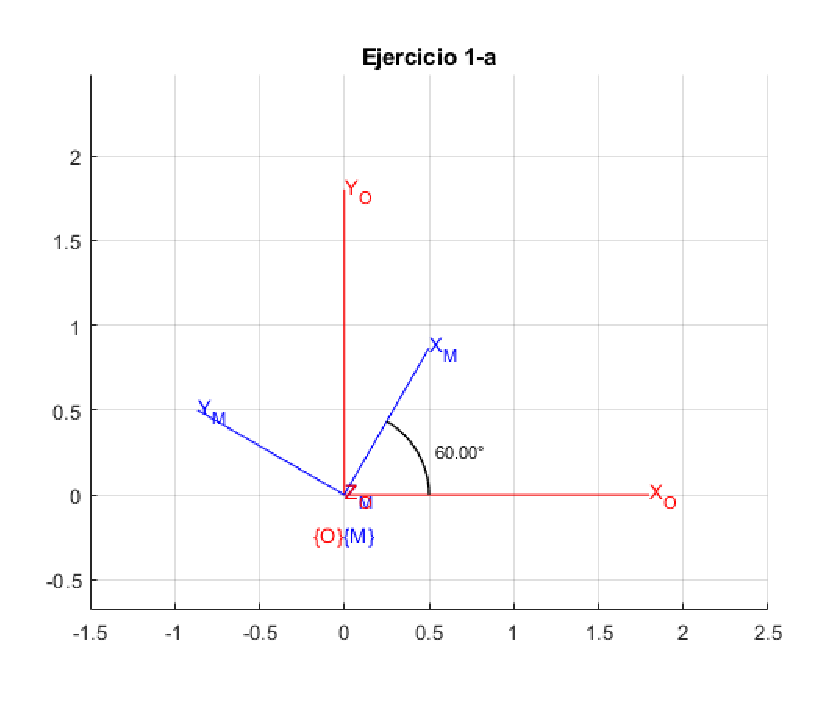
\includegraphics{1-Ejercicio_1_a.pdf}}
%    \end{adjustbox}
%    \caption{Sistema O y Sistema M superpuestos con indicación de ángulo de rotación.}
%\end{figure}


%\begin{table}[H]
%    \centering
%    \begin{tabular}{|c|c|c|c|c|c|}
%    \hline
%    Sistema & $\theta$  & $d$           & $a$    & $\alpha$ & $\sigma$ \\ \hline
%    1       & $q_1$     & $199.2$       & $200$  & 0        & 0        \\ \hline
%    2       & $q_2$     & $59.5$        & $250$  & 0        & 0        \\ \hline
%    3       & $0$       & $q_3$         & $0$    & 180°     & 1        \\ \hline
%    4       & $q_4$     & $37.5$        & $0$    & 0        & 0        \\ \hline
%    \end{tabular}
%    \caption{Parámetros DH alternativos.}
%    \label{parametros DH2}
%\end{table}

\end{document}